%\documentclass[12pt,notitlepage,a4paper]{article}
\documentclass[a4paper,11pt,floatfix,authordate1-4,twocolumn]{revtex4-1}

%\usepackage{times} % Times font
\usepackage{palatino} % Palatino font
\linespread{1.05} % A little extra line spread is better for the Palatino font
%\usepackage[T1]{fontenc}

\usepackage{caption}
\usepackage{graphicx} % Required for including images
\usepackage{setspace}
\usepackage{amsfonts, amsmath, amsthm, amssymb} % For math fonts, symbols and environments
\usepackage{xfrac}

%\usepackage[labelfont=bf]{caption} % Make figure numbering in captions bold
\usepackage[top=1.2cm,bottom=1.0cm,left=2.0cm,right=2.0cm]{geometry} % Reduce the size of the margin

% Select what to do with todonotes: 
% \usepackage[disable]{todonotes} % notes not showed
\usepackage[draft,colorinlistoftodos,bordercolor=white,color=orange!60,textsize=footnotesize]{todonotes}   % notes showed

% Select what to do with command \comment:  
% \newcommand{\comment}[1]{}  %comment not showed
\newcommand{\comment}[1]
{\todo[color=green!40]{\sffamily #1}} %comment showed

% Select what to do with command \reference:  
% \newcommand{\reference}[1]{}  %reference not showed
\newcommand{\reference}[1]
{\todo[color=blue!40]{\sffamily #1}} %reference showed

% Select what to do with command \wrong:  
% \newcommand{\wrong}[1]{}  %wrong not showed
\newcommand{\wrong}[1]
{\todo[color=red!70]{\sffamily #1}} %wrong showed


\hyphenation{poly-glu-ta-mine} % Specifies custom hyphenation points for words or words that shouldn't be hyphenated at all


%\linespread{1.3} % "one-and-a-half linespacing" see http://en.wikibooks.org/wiki/LaTeX/Text_Formatting#Line_Spacing
%\linespread{1.6} % "Double linespacing"

\begin{document}

\title{Computational clarification of the molecular mechanism that allows\\
 determining the number of growing ends in polyglutamine aggregation}

\author{Aniruddha Bapat}
\author{Markus S. Miettinen}
\email[Author to whom correspondence may be addressed. ]{\tt markus.miettinen@iki.fi}
\affiliation{Freie Universit\"at Berlin Fachbereich Physik}

\date{\today}

\begin{abstract}
{\bf Abstract.}
We use a combination of all-atom and coarse grained simulations
to study the molecular details of an assay used for
determining the number of growing ends in polyglutamine
aggregation kinetics experiments.
%
To this end we perform (all-atom) simulations of
polyglutamine fibrils tagged with biotin-PEG-polyglutamine,
as well as (coarse grained) simulations of
the interaction of these fibrils with streptavidin.
%
For the latter part we develop a model for biotin
within the Martini framework.


\vspace{14pt}
{\it
* This work is progressed and discussed openly at \url{markussmiettinen.github.io/biotinPEGpolyQ}.
Following the approach established in the NMRlipids project
(\url{nmrlipids.blogspot.fi/2013/07/on-credits.html}),
everyone is invited to join the discussion and make contributions.
The manuscript will be eventually submitted to an appropriate peer reviewed journal, and
everyone who has openly contributed, will be offered coauthorship.
The final decision on authorship will be to the invited individuals themselves;
they should base their decision on self-assessment of their scientific contribution to the project.
%
We hope that all communications would be written such that they are assignable
to a person and affiliation, as this will remove unnecessary ambiguity upon publishing.
%
Finally, it is the responsibility of contributors to make sure that in case they write something in which other people have had a scientific contribution (such as supervisors writing comments based on discussions with their students), the identities of all contributors should be made known. These secondary contributors will also be offered coauthorship in the manuscript.
%
As the project is part of A.~Bapat's studies, he will be the first author;
otherwise, the author names are alphabetically ordered with M.~S.~Miettinen as the corresponding author.

* This manuscript describes the current status of the project.
%
We use four kinds of comments to point out issues:
1) general comments \comment{\textbackslash comment} (green),
2) todo items \todo{\textbackslash todo} (orange),
3) asking references to be added \reference{\textbackslash reference} (blue), and
4) pointing out mistakes \wrong{\textbackslash wrong} (red).
%
The list of open issues is in the end of the manuscript.
}
\end{abstract}

\maketitle

\thispagestyle{empty}

\section{Introduction}
Nine inherited neurodegenerative diseases, including Huntington's disease,
are found to be caused by proteins having a polyglutamine (polyQ) repeat
exceeding a threshold of (typically) 35+ consecutive glutamines~\cite{Williams:2008a,Hands:2010a}.
%
As the glutamines in the polyQ repeat are in DNA coded using exclusively the CAG nucleotide triplet,
the {\it polyQ diseases} are also known as the {\it CAG triplet disorders}.
%
The onset and severity of polyQ diseases
correlate with the length of the polyQ sequence, and in the neuronal
cells of the deceased patients fibrillar aggregates rich in polyQ are found. 
%
Furthermore, as the proteins causing the diseases lack common
features other than the polyQ tract,
it is thought that associated with this tract is some
common molecular property that is critical for understanding all the diseases.

In our previous simulational work on polyQ we have focused on understanding the molecular
details of how its aggregation is initiated.
With all-atom explicit water molecular dynamics simulations and docking calculations
we have estimated the relative feasibility of
six different suggested
conformations~\cite{Perutz:1994a,Perutz:2002a,Sikorski:2005a,Zanuy:2006a,Fiumara:2010a,Kar:2011a}
of a $\mathrm{Q}_{40}$ peptide to be the aggregation-initiating conformer.
Our simulations strongly support $\beta$-hairpin-containing conformers,
and highlight the importance of side chain interdigitation between
hairpins~\cite{Miettinen:2012a,Miettinen:2014a}.



\subsection{Why is it important to know the number of growing ends?}
Many molecular details of  an amyloid formation process
can be assessed through aggregation kinetics experiments,
in other words, by measuring the concentration of aggregated peptides
as  a function of time,
and analyzing these data using nucleated growth polymerization theory~\cite{Ferrone:1999a}.
%
This applies not only to polyQ, but also to
understanding the aggregation of peptides linked to
other amyloid diseases, such as Alzheimer's or Parkinson's.
%
%This approach allows, for example, determining the size of the initiating nucleus.
%
A measure of particular interest here is
%However, in order to understand further molecular details of the amyloid growth process,
%it is very useful to know
the rate at which new peptides are being added to the growing fibril;
%
for example, when combined with molecular dynamics simulations, this
information can be used to assess which molecular structures can initiate the
aggregation process~\cite{Miettinen:2014a}.
%
Quantitative determination of this rate, however, requires determining the number
of growth sites (growing ends) in a kinetics experiment~\cite{Ferrone:1999a}.


\subsection{The assay used when experimentally determining the number of growing ends}
To determine the number of growing ends in a polyQ aggregation experiment,
biotinylated polyQ molecules (Fig.~\ref{Fig:sketch}) are used~\cite{bhattacharyya:2005a,onuallain:2006a}.
%
In the experiment one incubates a previously unknown number of preformed seeds (fibril fragments)
of non-biotinyled polyQ in a bath of biotinylated polyQ.
%
After incubation one adds Eu-streptavidin.
The streptavidin binds to biotins and
the europium allows concentration determination through fluorescence.
%
The key feature of the assay is that it can be demonstrated~\cite{onuallain:2006a}
that, for some unknown reason, only one streptavidin appears to be bound per growing end:
The Eu-fluorescence saturates orders of magnitude faster than the aggregation
process itself, and the values for the concentration of growing ends
are highly reproducible.
%
\begin{figure}[!htb]
%\vspace{-6pt}
\centering
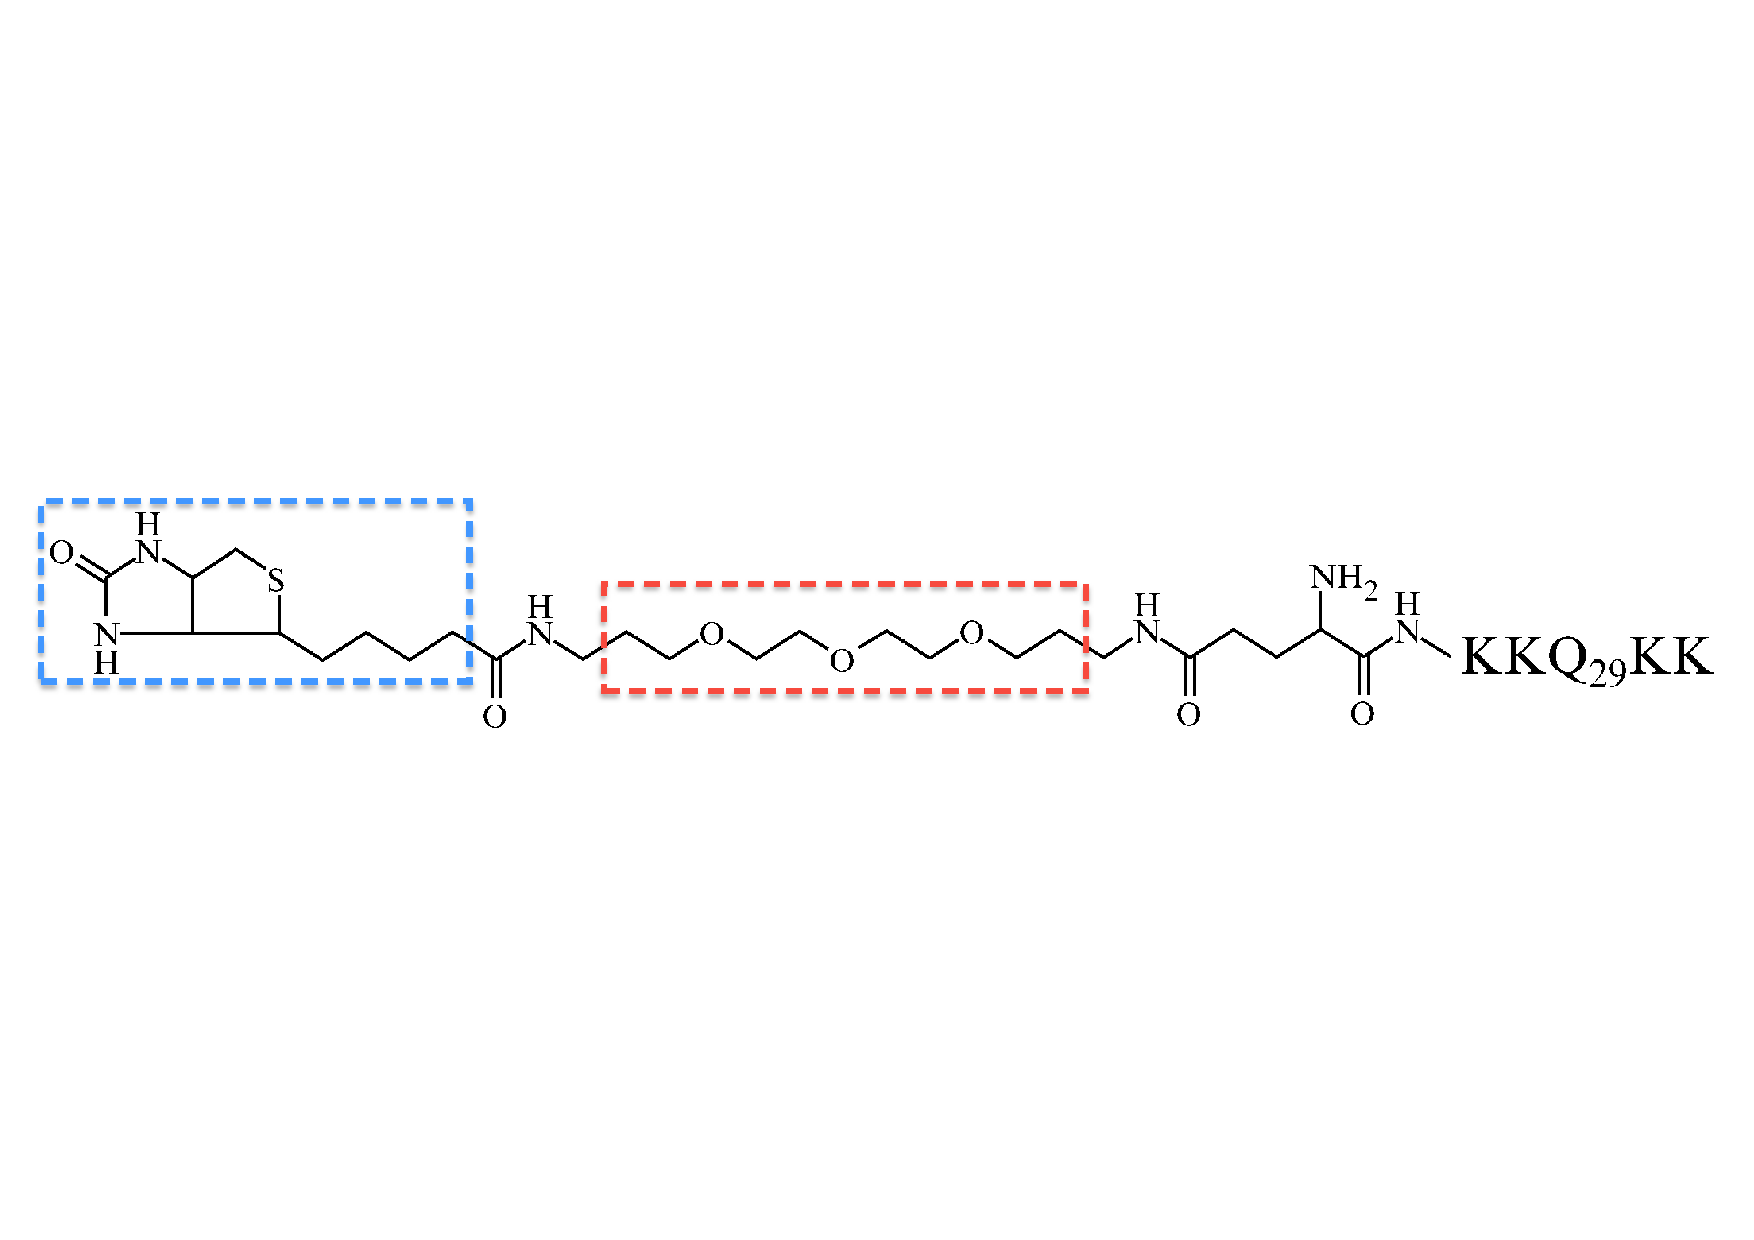
\includegraphics[width=\columnwidth]{../Figs/biotinylatedPolyQ_2.pdf}
\caption{\label{Fig:sketch}\footnotesize
Structure of the biotinylated polyQ,
highlighting the biotin tag (blue), and
the PEG linker (red).
}
\end{figure}


\subsection{Hypothesis on the molecular mechanism}
Based on the experimental findings~\cite{bhattacharyya:2005a,onuallain:2006a}, it appears that
any biotins on the biotin-PEG-polyQ chains within the fibril are for some reason inaccessible to binding by streptavidin,
in other words, only the biotin on the last bound molecule will bind a streptavidin and give signal;
although there is some experimental support for this hypothesis,~\footnote{
Personal communication from professor Ronald Wetzel
and from Dr. Elizabeth Landrum, University of Pittsburgh.
}
the molecular mechanism remains unknown.~\footnote{
Private communication with professor Ronald Wetzel, University of Pittsburgh.
}
%

\subsection{Clarification of the molecular mechanism using all-atom simulations}
To test the hypothesis, all-atom explicit water simulations
with three different setups will be run:
(1) single biotin-PEG-polyQ molecule in the growing end of a pure-polyQ fibril,
(2) single biotin-PEG-polyQ molecule in the middle of a pure-polyQ fibril, and
(3) fibril comprising only biotin-PEG-polyQ molecules.

Comparing the conformational distribution of the biotin-PEG tag between cases (1) and (2) will reveal
if (and to what extent) the position of the tag within the fibril affects its availibility
to strept\-avidin. A possible scenario is, for example, that when the tag is in the middle of the
fibril, it will more strongly bind to the fibril surface than
when being located at the growing end.
%
Case (3) will reveal to what extent neighboring biotin-PEG tags interact with one another;
do they, e.g.,
fold in such a way as to prevent them from being available for streptavidin
binding.

\subsection{Clarification of the molecular mechanism using coarse grained simulations.}
Streptavidin is a tetrameric protein, whose each monomer comprises over 100 amino acids.
Its sheer size thus prohibits direct all-atom simulations of
its interaction with the biotinylated polyQ fibril.
%
We, therefore, resort into coarse grained simulations using the Martini model~\cite{Marrink:2007a}
to study the interaction of the streptavidin tetramer with
the same three fibril systems that we studied with the all-atom model.
%
These simulations will allow us to confirm if the differences found in
the biotin-PEG tag conformations using the atomistic model also
translate into differences with regards to the access of biotin into the binding
pocket of streptavidin.

\section{Methods}

\subsubsection*{Building the all-atom model}

\todo[inline]
{{\bf Aniruddha},
start writing here a description on how you are
building the fibril.}

All-atom explicit water simulations
with three different setups will be run:
(1) single biotin-PEG-polyQ molecule in the growing end of a pure-polyQ fibril,
(2) single biotin-PEG-polyQ molecule in the middle of a pure-polyQ fibril, and
(3) fibril comprising only biotin-PEG-polyQ molecules.
To guarantee the reliability of the results,
10 independent simulations for each setup will be performed.

There is no existing molecular dynamics force field for the biotin-PEG-polyQ.
%
However, within the CHARMM force field family, models for both the biotin~\cite{Izrailev:1997a}
and PEG~\cite{Lee:2008b} have been created. Thus a force field for the biotin-PEG-polyQ
could, in principle, be built simply by joining these existing building blocks of
biotin and PEG to a polyglutamine chain described using the CHARMM36~\cite{Best:2012b}
force field.

Having said that, the above mentioned works on biotin and PEG are rather old, and using
the powerful modern tools for creating force fields for small molecules,
such as CGenFF~\cite{Vanommeslaeghe:2012a}, to create a CHARMM36-compatible
biotin-PEG from scratch, will possibly lead to a more reliable result.

\comment{\textbackslash We have recently successfully used a PEG model based 
on work modification by Shang et al. [J. Phys. Chem. B 2008, 112,
2888−2900] to the GROMOS 45a3, see dx.doi.org/10.1021/la404684r.
The model works (surprisingly) well reproducing even anoumalous
temperature dependence (increasing of order parameters with increasing
temperature, see Fig. 5.). This may be useful if you find compatible models
for other molecules.} 

\todo[inline]{
{\bf Scaling plots (DL: Oct 25th).}
To apply for computing resources we need to run scaling tests.
For this we need a system that is as close to the actual system we will work on as possible.
Naturally, we can not include biotins and PEGs yet, but pure polyQ will suffice here.
To this end we must:
{\bf (1)} estimate the size of the fibril (number of Qs, number of waters) we need to simulate,
{\bf (2)} build a system of this size (does not need to be a fibril),
{\bf (3)} simulate with varying number of cores.
}



\subsubsection*{Building the coarse grained model}
As in the all-atom case, there is exists no biotin-PEG-polyQ in Martini~\cite{Marrink:2007a}.
%
However, Dr. Luca Monticelli's group has recently developed a Martini model for PEG~\cite{Rossi:2012a}.
In addition, we have developed a model of glutamine that allows fibril formation
by allowing for interdigitation of stacked hairpins---a
feature that was prevented by the shape
of the standard Martini~\cite{Monticelli:2008a} glutamine,
but which I have shown is highly important in
correctly describing polyQ aggregation and
fibril formation~\cite{Miettinen:2014a}.

%
Thus the only part missing is the biotin, which we shall parametrize
in such a way as to reproduce the conformational distributions
in our all-atom simulations of the biotinylated polyQ fibrils.

Notably, we are not going to focus on carefully parametizing
the interactions of biotin with the streptavidin binding pocket;
we are only interested the ability of biotin to enter the pocket,
not its actual binding affinity.
%
(However, the biotin model we develop will probably be useful
as a starting point for other researchers that wish
to study the biotin--streptavidin interaction.)


\section{Results}


\section{Discussion}

\todo[inline]{
Should probably {\bf discuss the recent paper by de Pablo~\cite{Fluitt:2015a}},
where they show how (badly) current MD FFs describe polyQ in solution.
Not a crucial problem for us here (which we should point out), as our polyQ is in the fibril,
but a worthwhile work nonetheless.
}

%------------------------------------------------
%\pagebreak
\section*{Bibliography}

%----------------------------------------------------------------------------------------
%	BIBLIOGRAPHY
%----------------------------------------------------------------------------------------

%\newpage



\setstretch{0.5}
\bibliography{bbRefs.bib}

\begin{figure}[!hb]
\centering
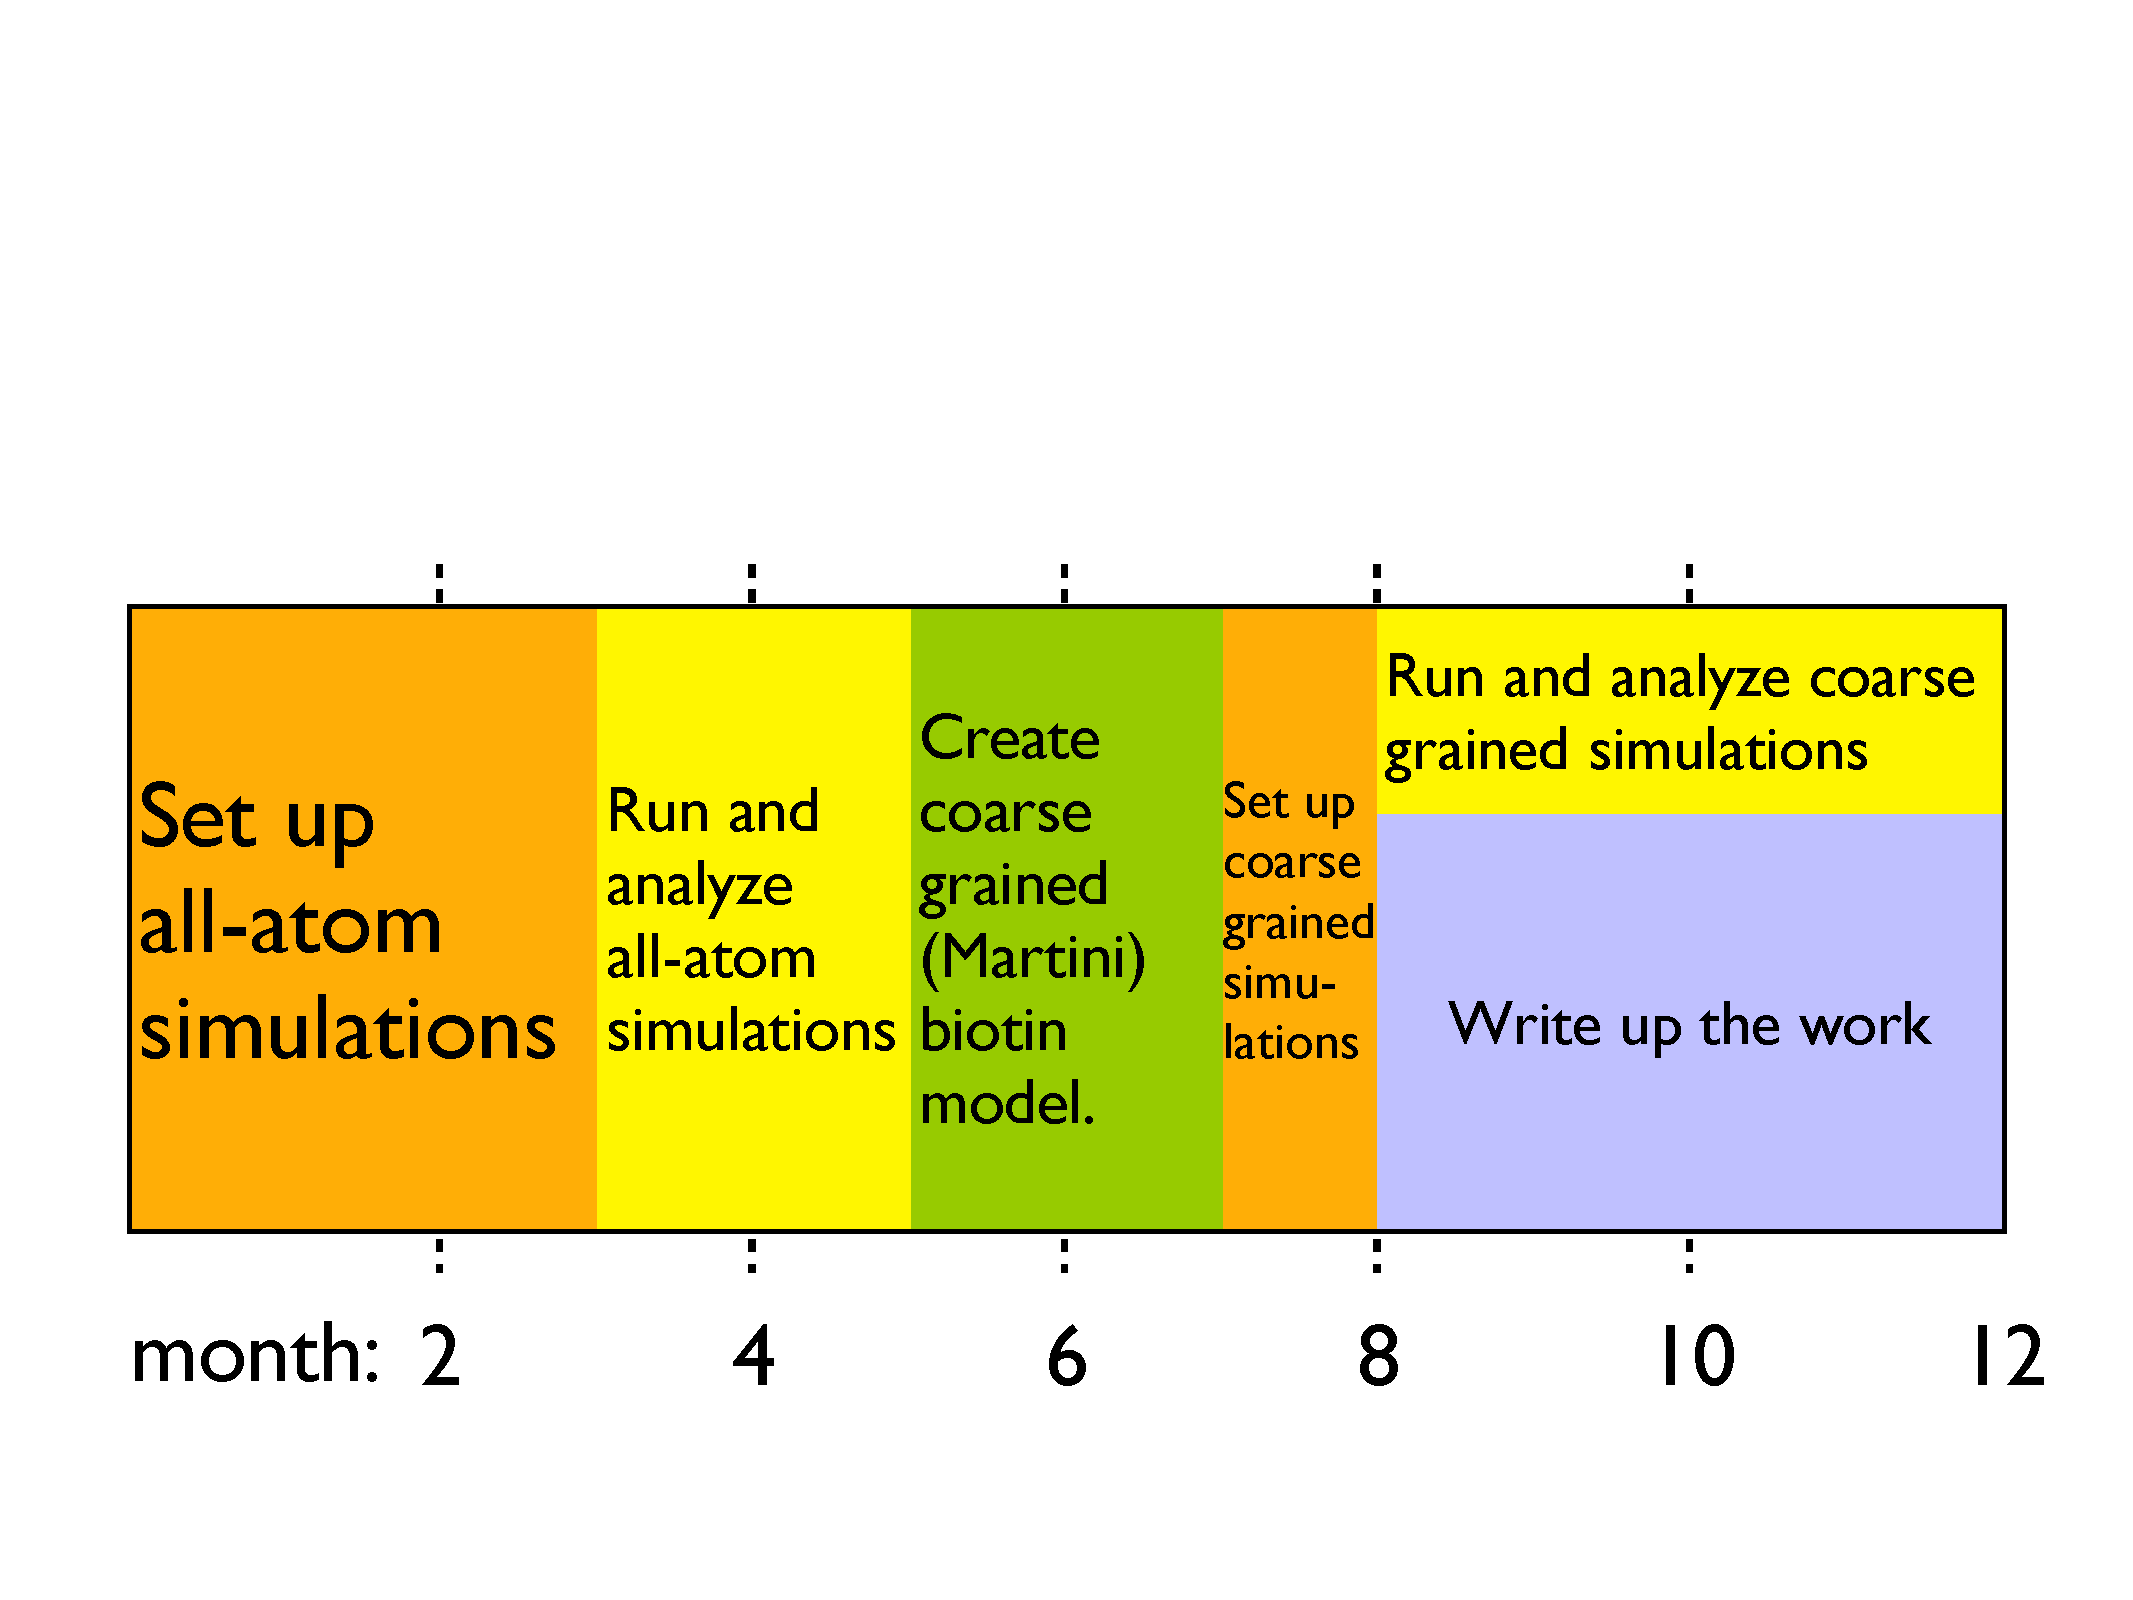
\includegraphics[width=\columnwidth]{../Figs/timetable.pdf}
\captionsetup{labelformat=empty}
\caption{\label{Fig:timetable}\footnotesize
Rough work- and timetable for the planned 12 months
duration of the project.
}
\end{figure}

\listoftodos[Open issues]

\end{document}
